% !Mode:: "TeX:UTF-8"

\chapter{分层光网络下的并行路由优化算法研究}
\section{引言}
  随着视频流、云计算服务和移动应用的普及,互联网的流量不断增加[],业务量的持续增长给互联网的传输带来了巨大的挑战,为了满足日益增长的容量要求,波分复用(WDM)系统已部署在骨干网络,其每个通道带宽高达40 GB/s或100 Gb/s。现在,400 Gb/s的带宽接口已经在实验室[2]实现,此外,为了满足不同的数据速率服务异构的流量类型,混合线路速率(10/40/100Gb/s)的WDM系统也已经部署。因此,WDM光网络视乎为大流量业务传输提供了一个既实际又高效的解决方案。
  然而,传统的WDM光网络严格遵循ITU-T的固定均匀间距和网格(通常为50)GHz或100千兆赫)[],这样会导致低效的频谱利用率,比如,一个较大的波长可能会被分配给一个低速率的业务,即使这个业务根本就不能占满整个波长。很明显,传统WDM光网络的不灵活和粗粒度的带宽控制会导致显著的频谱浪费,限制了提高其网络容量的潜力。
  为了应对WDM网络的低敏捷性和频谱浪费问题,近年来,弹性光网络(EON)的架构被提出,在EON架构中,存在细粒度的带宽间隙(比如,12.5GHZ),他比WDM网络所遵循的ITU标志的50GHZ或者100GHZ的带宽粒度要小很多,而且,这些带宽间隙可以根据需要被组合在一起以提供更宽的通道。所以为了提高带宽利用率,在EON中存在混合速率,每个速率的业务需要不同数量的频谱间隙数量。理论上,EONs能够灵活地提供各种速率,但是在实际中,EONs却可能只含有很少的速率种类,这主要是因为:第一,随着频谱的增加,频谱碎片和管理复杂度将显著增加。第二,实际的EON从较低的线路费率升级到更高的线路费率,并存大量速率的情况已经很少见了。
  为了在EON网络中加入业务,控制平面必须在网络中找到一条路径,同时,还需要在此路径上的链路上分配足够的频谱带宽,来创建一个合适的端到端光路连接,这被称为路由和频谱分配(RSA)问题,EONs中的RSA问题比传统的在WDM网络中的路由和波长分配(RWA)问题更具有挑战性,传统的RWA解决方案[][]在EONs中已经变得不再适应了。在EONs中一个业务需求可能需要多个连续的频谱间隙,而且由于缺少全光谱转换器,每条光连接的频谱从它的源节点到它的目的节点 ,在所经过的链路上保持不变,这被称为频谱连续性限制。
  根据流量模式,RSA问题可以进一步分为静态RSA问题和动态RSA问题。静态的RSA问题出现在网络规划阶段,其中流量需求是已知的,这样可以离线计算出最优或者接近最优的RSA解,动态RSA问题是指在实时业务情况下光通路的路由选择和波长分配的优化问题,在动态RSA问题中,业务随机的到达和离开光网络,而且当业务到达网络时,控制平面需要在短时间内找到RSA解来安排业务。动态RSA问题比静态RSA问题更具有挑战性,因为业务需求随机到达和离开,网络状况随时发生变化,而且要求控制平面反应实时。
 链路代价表示路由路径选择这一条链路所需要的代价,链路代价可以设置为链路的距离,延迟,租用链路需要的费用等等,业务的路由代价表示业务路径经过的链路的代价总和,路由代价反应了路由路径的优劣程度,如果链路代价设置为延迟,则路由代价越小表示路由整体延迟较小,如果链路代价设置为1,则路由代价越小,表示路径经过的跳数越小,使用的链路资源越小。
 本章考虑在EONs中解决动态RSA问题,设计出带跳限约束下的基于分层图的动态路由优化算法来优化整体路由代价,分别考虑无权图和带权图上的算法GPU加速设计,GPU并行版本达到平均近6倍的算法加速比,实验与分层图上的传统算法比较,显示该算法过程在短时间内能够大量的优化路由代价,并且由于路由选择较优,使用网络资源较少,最终网络阻塞率表现也有显著的提高,实现了快速的路由代价优化和整体的阻塞避免。
\section{问题描述}
\subsection{EONs中动态RSA问题}
  在动态场景中,业务的到达时间和服务时间都是随机的,当业务到达网络时,SDN控制层需要找到可行的路径,并且为路径分配合适的频谱资源。由于EON的物理限制,RSA问题的解需要满足以下限制:
%\begin{enumerate}[(i)]
第一,传输距离限制:光信号的传输质量会随着传输距离的增加而下降,为了在目的点顺利恢复光信号,光链路的传输距离需要小于一个阈值$D_max$,为了简化设计,本文假设每一条链路的长度相同,都是一个单位,那么传输路径的跳数需要小于阈值$D_max$。
第二,频谱连续性限制:每条光连接的频谱从它的源节点到它的目的节点 ,在所经过的链路上保持不变。
第三,频谱不重叠限制:同一光纤链路中的频谱不能分配给不同的光路。
第四,频谱邻近限制:频谱邻近约束保证分配给一个光路径的频谱必须是一个连续的部分。
 此外,为了限制路径对网络频谱的资源使用,我们为路径加入跳限约束,论文[]中对网络加入跳限约束,使得整体上阻塞率降低,此外,后面将讨论,加入跳限约束后能够简化GPU上代码的实现,使得算法可以提前结束,节省同步标记。
\subsection{分层网络模型}
  论文[]中提出一种分层图模型来解决WDM网络中的路由和波长分配问题,分层图模型将路由选择和波长分配问题统一到一起来,使得RWA问题变得简化,这种分层图模型也可以很容易推广到EONs的RSA问题中。
  我们使用有向图$N(V,E)$表示物理网络拓扑,其中$V={v_1,v_2,...,v_N}$表示节点集合,$E={e_1,e_2,e_3,...,e_M}$表示边集合,$e_k=(i_k,j_k)$表示边的头节点为$v_{i_k}$,边的尾节点为$v_{j_k}$。假设所有光链路具有相同的频谱范围$W=(F_{start},F_{end})$,其中$F_{end}-F_{start}=C$。EON所支持的速率集合为$R$,比如,$R={40Gb/s,100Gb/s,400Gb/s}$,每一种速率$r\in R$需要一个特定的频谱宽度$b_r GHz$。一个源节点为$s$,目的节点为$t$,速率为$r Gb/s$的业务被表示为$TD(s,t,r)$。
  下面我们讨论分层图的产生过程,假设第一个速率的为$r$的业务$TD_r(s,t)$到达网络,我们从可用的频谱切割出一块频谱大小为$b_r$的连续带宽分配给速率为$r$的业务,假设这块频谱的起始频率为$fs_{(r,1)}$,终止频谱为$fe_{(r,1)}$,那么$fe_{(r,1)}-fs_{(r,1)}=b_r$,我们把所有物理链路上频谱范围$(fs_{(r,1)},fe_{(r,1)})$,从链路上“割”下来,把“割”下来的部分组成一个新的虚拟网络$N^{(r,1)} (V^{(r,1)},E^{(r,1)})$,在这个新的网络中每条链路的频谱范围都是$(fs_{(r,1)},fe_{(r,1)})$,这样切割下来之后,原来的物理网络的频谱范围更新为$(F_{start}+b_r,F_{end})$。
  然后在这个复制出来的图上为业务求一条最短路径$p$,那么容易知道路径$p$一定满足约束2,3,4,这样问题被简化为单纯的路由问题。要注意的是,这个虚拟图上频谱不能再分配给其他速率为$r'$的业务$TD_r'(s',t')$,即使$b_r'<b_r$,这是因为这样会产生大量的频谱碎片,使得频谱利用率下降,阻塞率降低,并且这样会使得问题变得更加复杂化,所以这些分割出来给速率$r$的频谱,将继续被分配给速率为$r$的业务。当下一个速率为$r$的业务$TD_r (s'',t'')$到达网络后,他首先在图$N^{ (r,1)}(V^{(r,1)},E^{(r,1)})$中寻找路径,如果找到合适的路径则加入网络并且更新路径链路的可用频谱为0;反之,如果他在图$N^{(r,1)} (V^{(r,1)},E^{(r,1)})$中没有找到合适的路径,那么算法会重新去”切割“物理拓扑得到虚拟网络$N^{(r,2)} (V^{(r,2)},E^{(r,2)})$,这样随着大量业务的动态的到达和离去,会产生大量的虚拟图,频谱资源已经大量地分布在各个虚拟图中,我们把这些虚拟图叫做分层图(layered Graph),现在RSA问题转化为在分层图中求解路由的问题,问题被简化。
  下图表示分层图示意,原图被切割成一个分层图集集合$L$,$L_i \in L$表示速率$i$的分层图集,如图所示,速率$k$的一共有$|L_k|$个图副本,每个子分层图占用频谱$(fs_{(r,1)},fe_{(r,1)})$,图中,点$v_i^{(r,l)}$表示速率$r$的第$l$层图上的第$i$号点。
$f_{()}$
\begin{figure*}
\setlength{\belowcaptionskip}{-0.5cm}
  \begin{center}
    {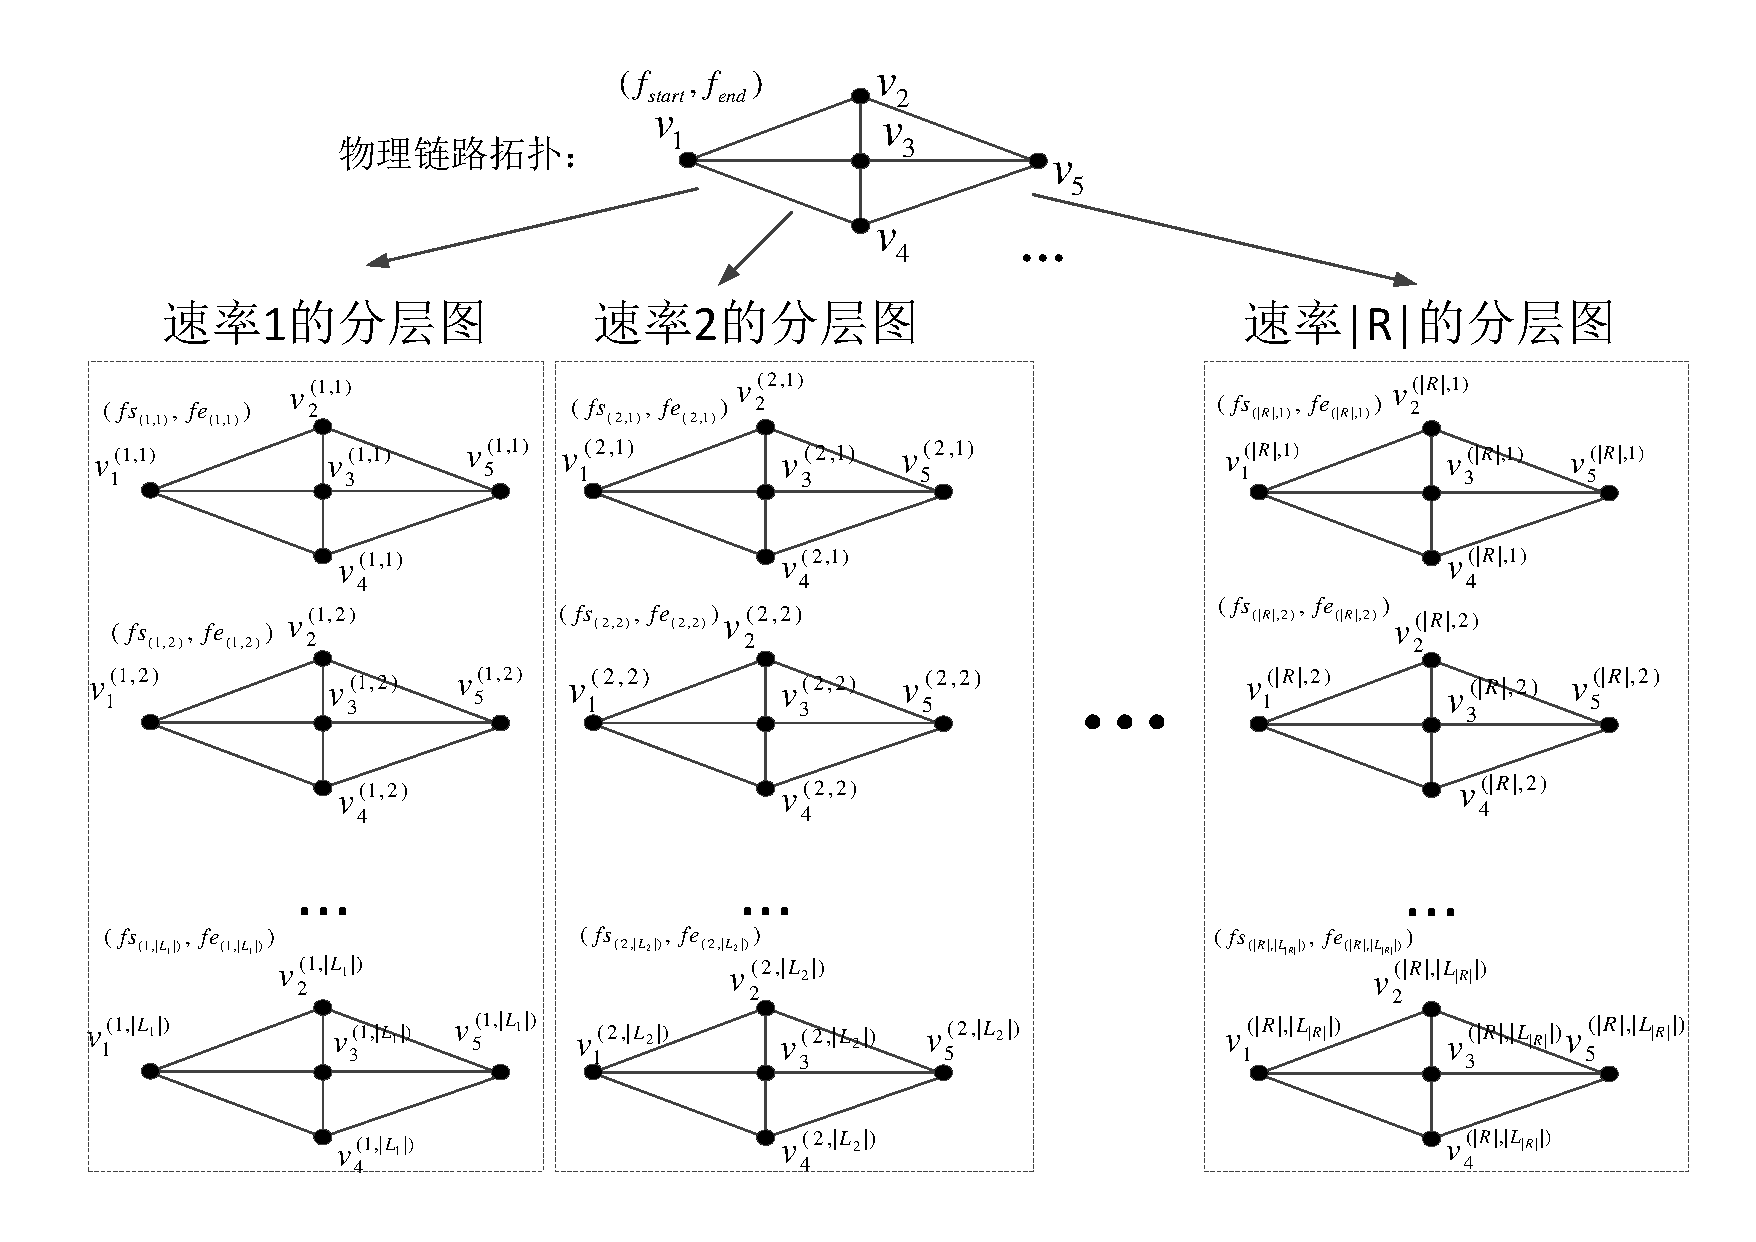
\includegraphics[width=1 \textwidth]{figures/LAYER.pdf}}
    \end{center}
  \caption{{\footnotesize{分层图示意}}}
  \label{layer}
\end{figure*}
\section{主要优化流程}
  根据前面的讨论,当一个速率为$r$的业务$TD_r(s,t)$到达网络时,一共有$L_r$个分层平面都可以用于此业务,也就是说如果在这些图当中都能为业务找到合适的路径的话,那么业务就有$L_r$条路径可供选择,我们可以选择代价最小的一条来优化路由。进一步,当有一批速率为$r$的业务集合$TD_r$到达网络时,如果大家都选择同一层加入的话,会出现大量的冲突,而且路由代价也会很大,但是由于现在有多个分层图平面可以选择,每个业务都有$L_r$条路径可以选择,这就给路由优化提供了可能,不同的业务需求可以选择不同层上的路径来进行路由,以使得总体路由代价减小,节省网络频谱资源,从而优化阻塞率。本节提出一个基于分层图的动态RSA优化算法流程,算法流程图如下所示:
 \begin{figure*}
\setlength{\belowcaptionskip}{-0.5cm}
  \begin{center}
    {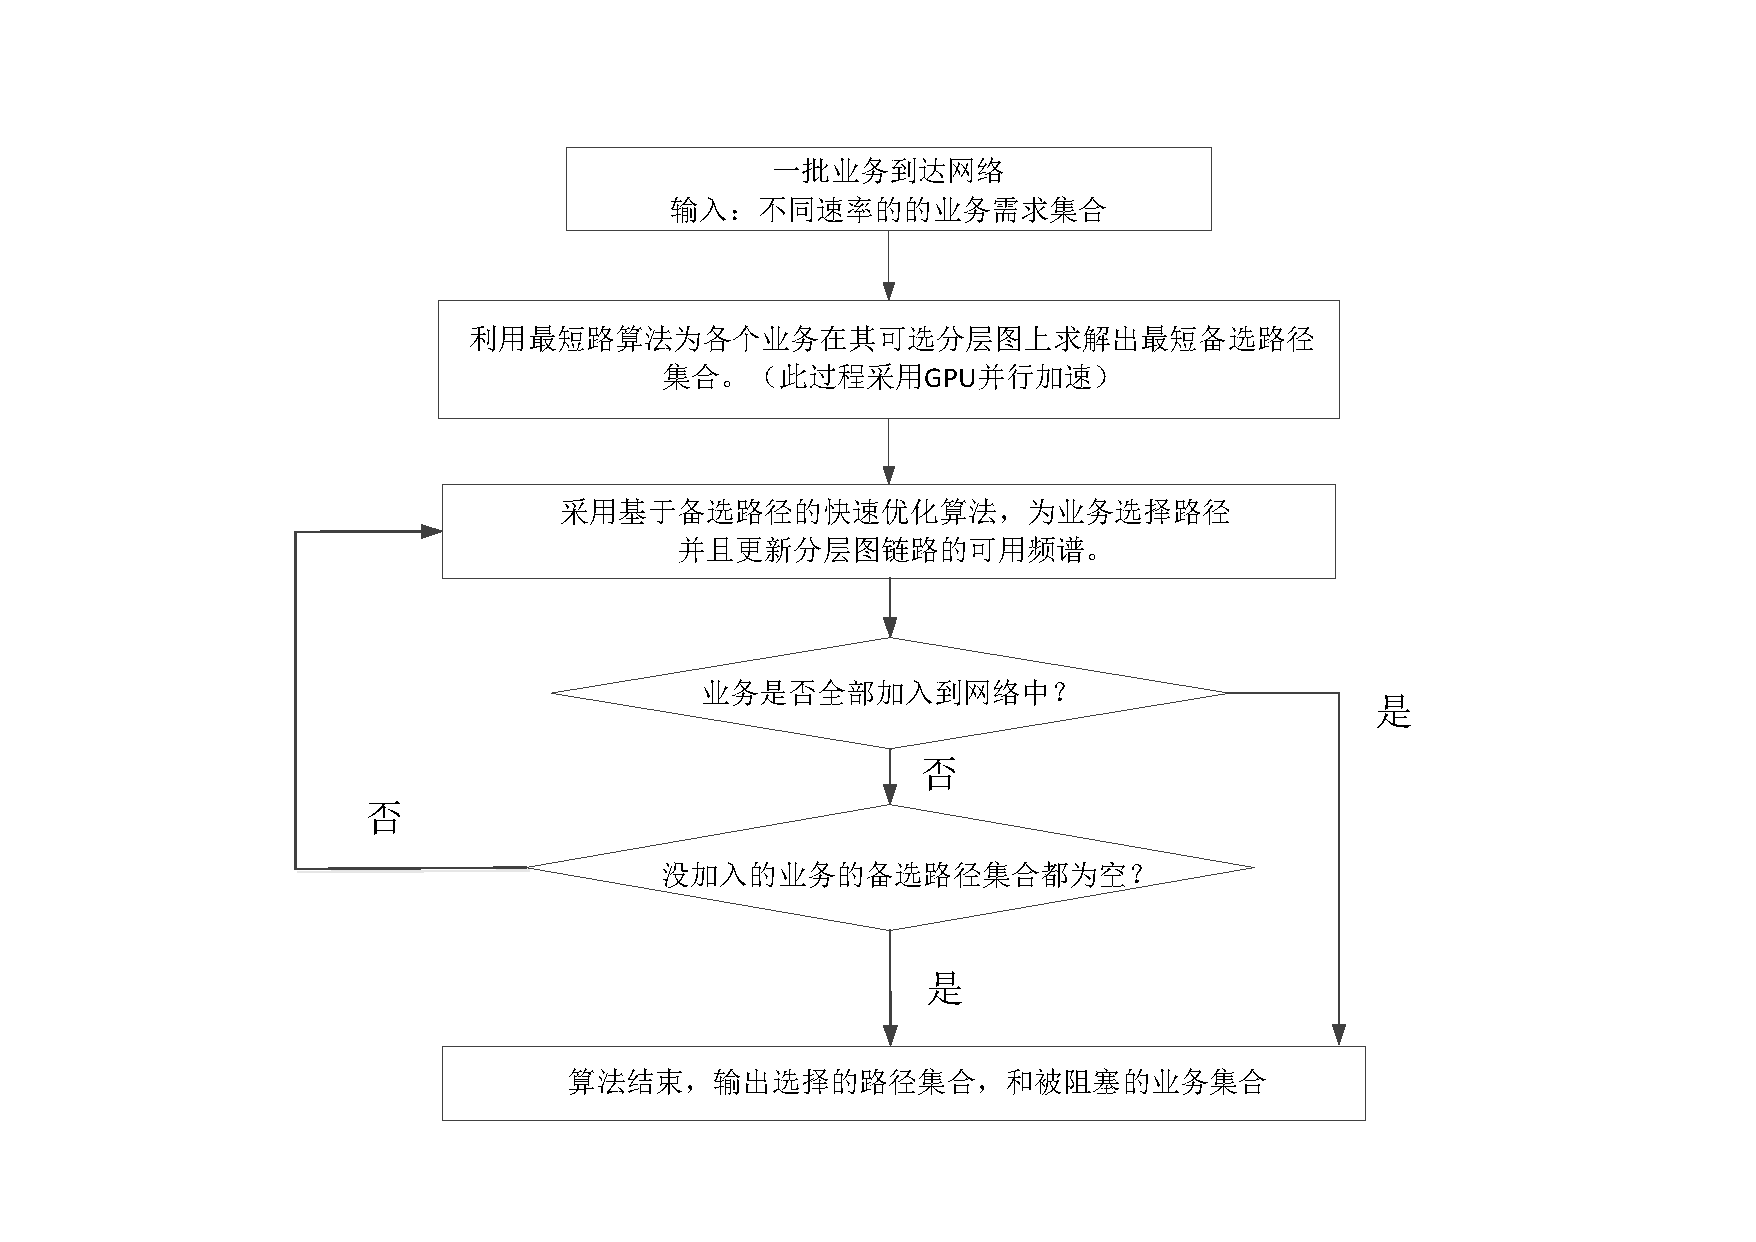
\includegraphics[width=1 \textwidth]{figures/bbprocess.pdf}}
    \end{center}
  \caption{{\footnotesize{算法优化流程}}}
  \label{bblayer}
\end{figure*}
 当一批业务到达网络时,对每一个业务在其对应速率的层上求出大量的备选路径,这个过程计算量较大,但是每一个拓扑层是独立的,所以可以采用并行算法来进行加速设计,后面**将讨论无权图和有权图上的两种基于GPU的路由加速算法来加速这个步骤,当备选路径都求出来了之后采用一种快速路径选择算法来把业务安排进网络,这个步骤采用一种简单贪心的启发式算法,由于备选路径较多,实验发现这种简单的贪心算法已经可以很好的优化路径代价了。当业务的路径确定后,如果每个业务都能加入到网络,那么本轮算法结束,如果还有剩余的业务没有被安排进网络,需要判断业务的备选路径集合是否为空,如果为空,则说明所有层都不能为业务求出路径,业务将被阻塞;反之,如果业务的备选路径集合不是空,则说明业务是因为和其他业务的路径冲突而导致不能被安排进网络,分层图中可能还存在其他可用路径,所以需要重新在分层图中计算路径,算法回到步骤二,对这些业务进行重新计算。
 步骤一的具体算法将在**结束,这里介绍步骤二的快速优化算法,快速优化算法的主要思想是根据求出来的备选路径为每个业务选择路径以使得整体路径代价最小,由于动态RSA环境下需要在短时间内安排好路径,所以为了提高计算速度,这里采用一种简单快速的贪心算法来进行解决。算法步骤如下所示:
\begin{algorithm}[htb] 
\caption{路径安排算法} 
\label{arrange} 
\begin{algorithmic}[1] 
\Require 
$N(v,E)$:分层图;
$P$:备选路径集合;
$TD$:业务需求集合;
\Ensure 
$AP$:加入业务的路径集合; 
\For{$T \in TD$}
\State {对$P_T$中的路径按照路径的代价进行降序排序}
\EndFor
\State {对$T$按照$P_T$中的最小路径代价进行排序}
\For{$T \in TD$}
\For{$p \in P_T$}
\If{路径$p$所对应分层图上的相应链路没有被占用}
	\State{把$p$加入到$AP$中,并更新$p$所对应的分层网络上的链路,跳出for循环,以继续为下一个业务选路}
\EndIf
\EndFor
\EndFor
\end{algorithmic} 
\end{algorithm}
 算法开始对每个业务的备选路径按照其代价进行降序排序,也就是每个业务优先会选择代价较低的备选路径。然后,再对业务按照其最小代价的路径进行排序,这样保证优先考虑代价小的业务。然后开始加入业务到网络,对每一个业务,遍历其已经排序好的备选路径,如果在相应分层图上路径包含的链路都是空闲的,则加入业务到网络中,更新分层图上的相应链路为占用状态,把这个路径$p$加入到集合$AP$中。最后算法输出路径集合$AP$,算法结束。
\section{无权图情况下的GPU算法设计}
  无权图情况下,路由的代价就是路径的跳数,跳数越少说明占用的网络资源越少,尽量优化路径的跳数可以节省网络资源,进一步的降低动态情况下的网络的阻塞。无权图情况下的路由算法一般使用BFS(宽度优先搜索)算法进行求解,BFS算法从目的节点最近的点开始,一层一层的进行扩展直到找到目的节点,每扩展一层跳数增加一条,扩展一层需要遍历大量的边,这些边的扩展操作是相互独立的,所以为算法提供了并行设计的可能性,在加上不同速率不同层上的路由求解上的并行,总体并行粒度是很大的,下面分别对不同的并行层次的设计进行讨论。
\subsection {相同速率业务的并行}
  如下图所示,对速率都为$r$的一批业务,在其可用的每个分层图上并行进行计算,在每个分层图上,具有相同源节点的业务组成业务组,因为他们的路径可以一起计算,对每一个业务组,在GPU上开辟$|E|$个线程对每一条边进行扩展操作,那么整个过程的的并行粒度为$|L_r|*|D_r|*|E|$,其中$|D_r|$为速率为$r$的业务组数量。
 \begin{figure*}
\setlength{\belowcaptionskip}{-0.5cm}
  \begin{center}
    {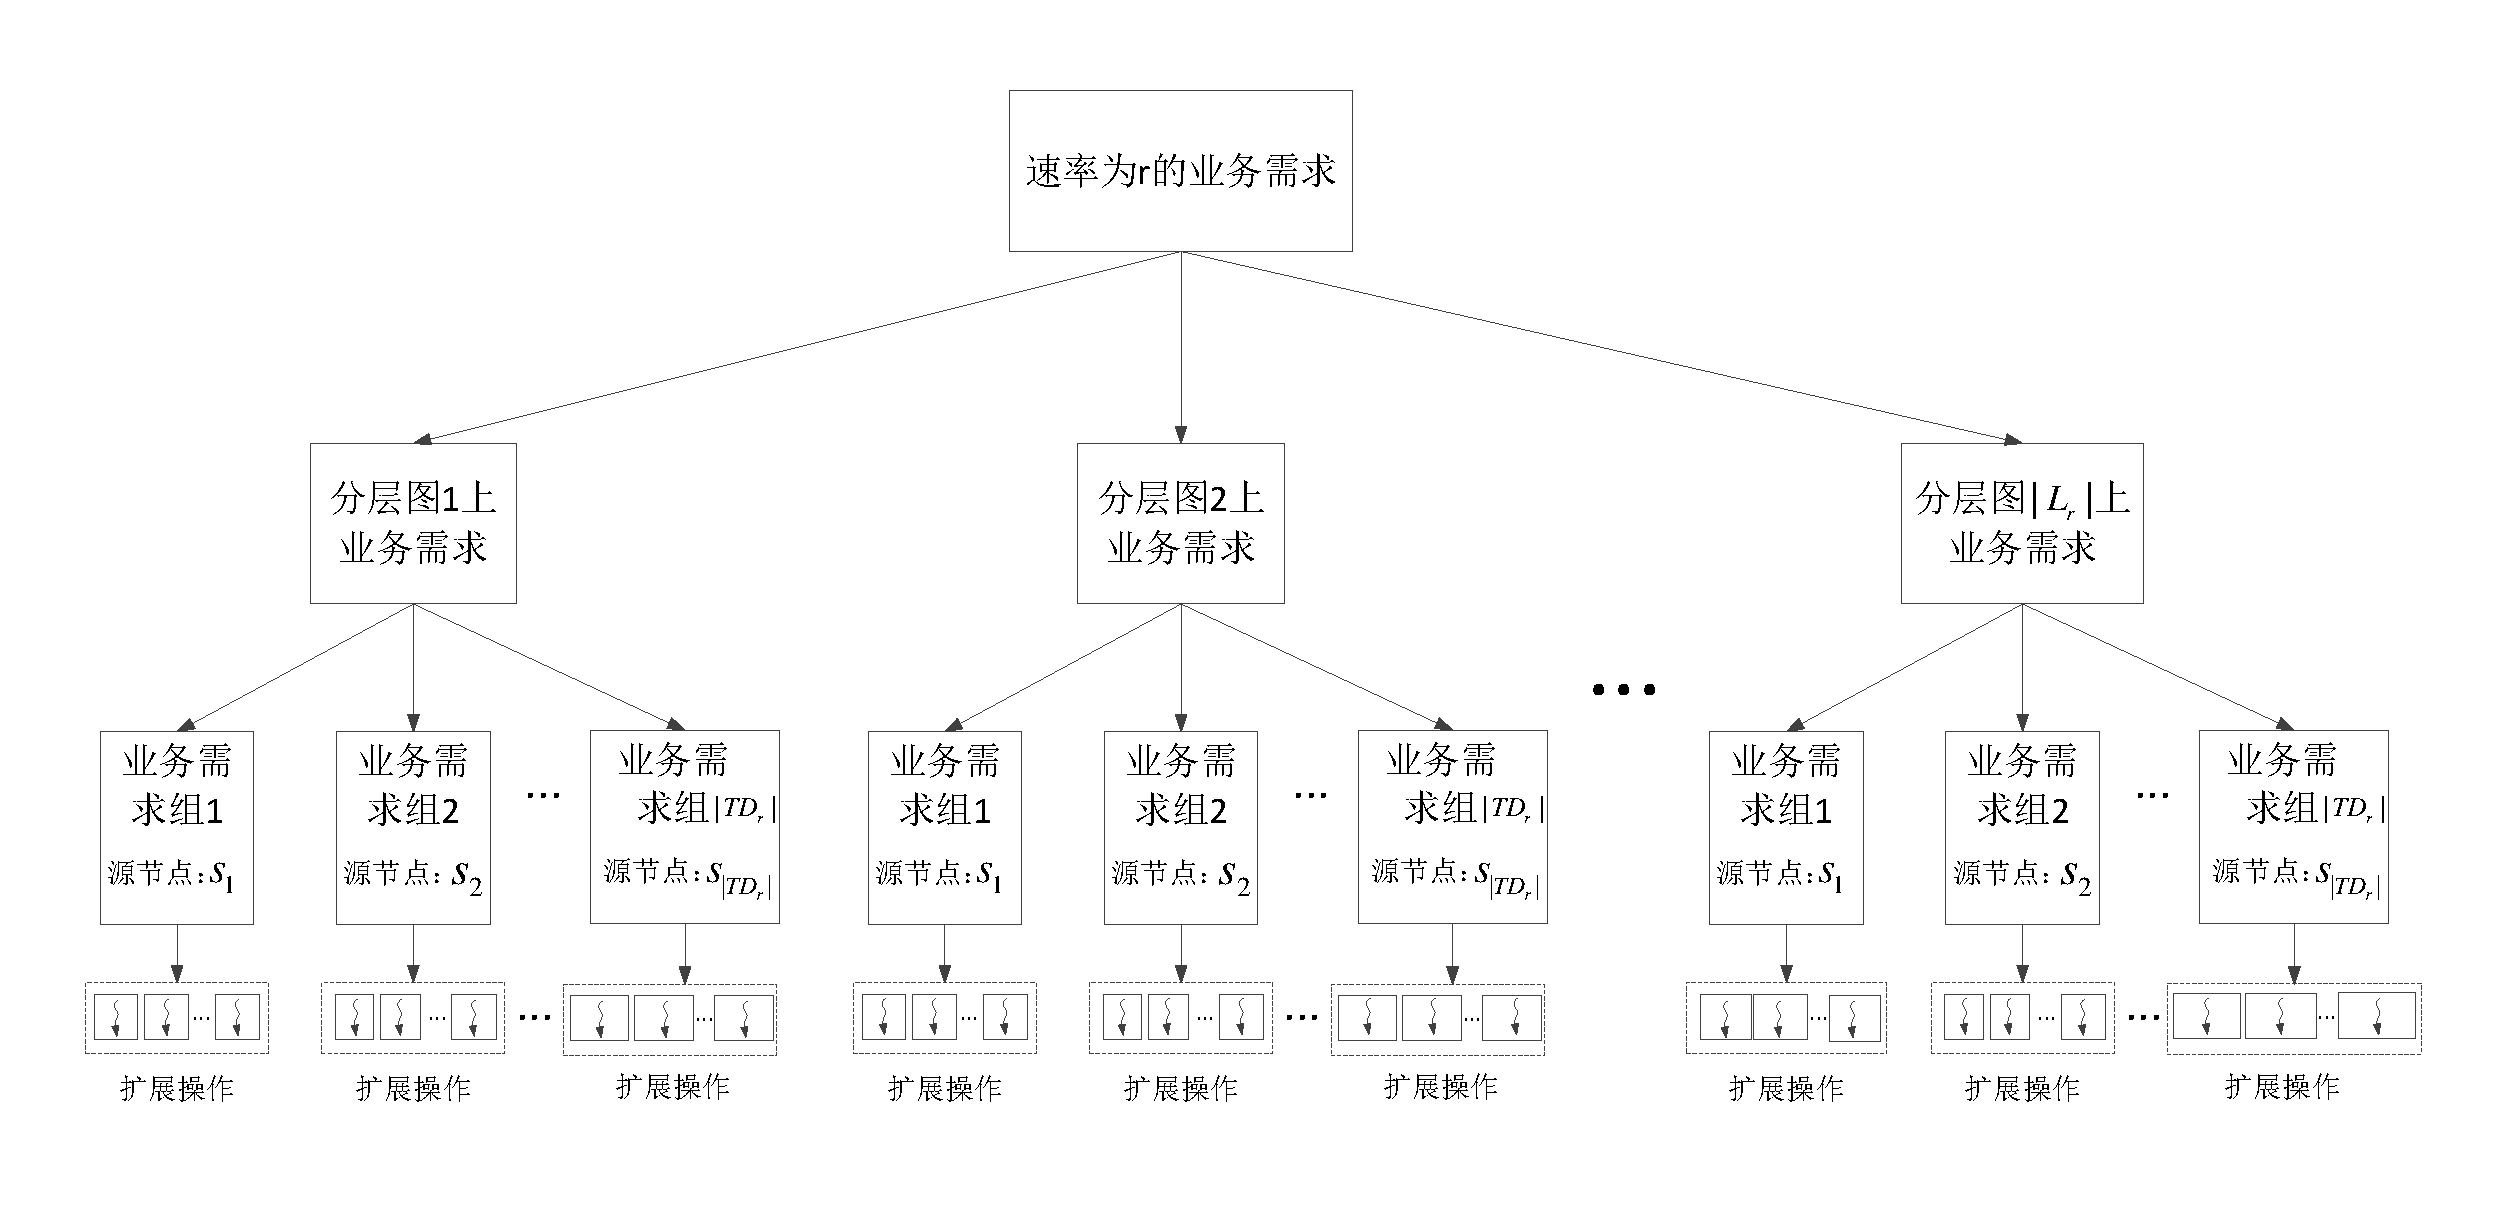
\includegraphics[width=1 \textwidth]{figures/bfs.pdf}}
    \end{center}
  \caption{{\footnotesize{bfs并行示意图}}}
  \label{bfs}
\end{figure*}
\subsection{不同速率间业务的并行}
  由于动态业务情况下每次到达网络的业务数和速率情况都是变化的,不同速率之间业务的并行不容易直接实现在一个kernel中进行,我们采用GPU提供的流并行进行并行设计。如下图所示:
 \begin{figure*}
\setlength{\belowcaptionskip}{-0.5cm}
  \begin{center}
    {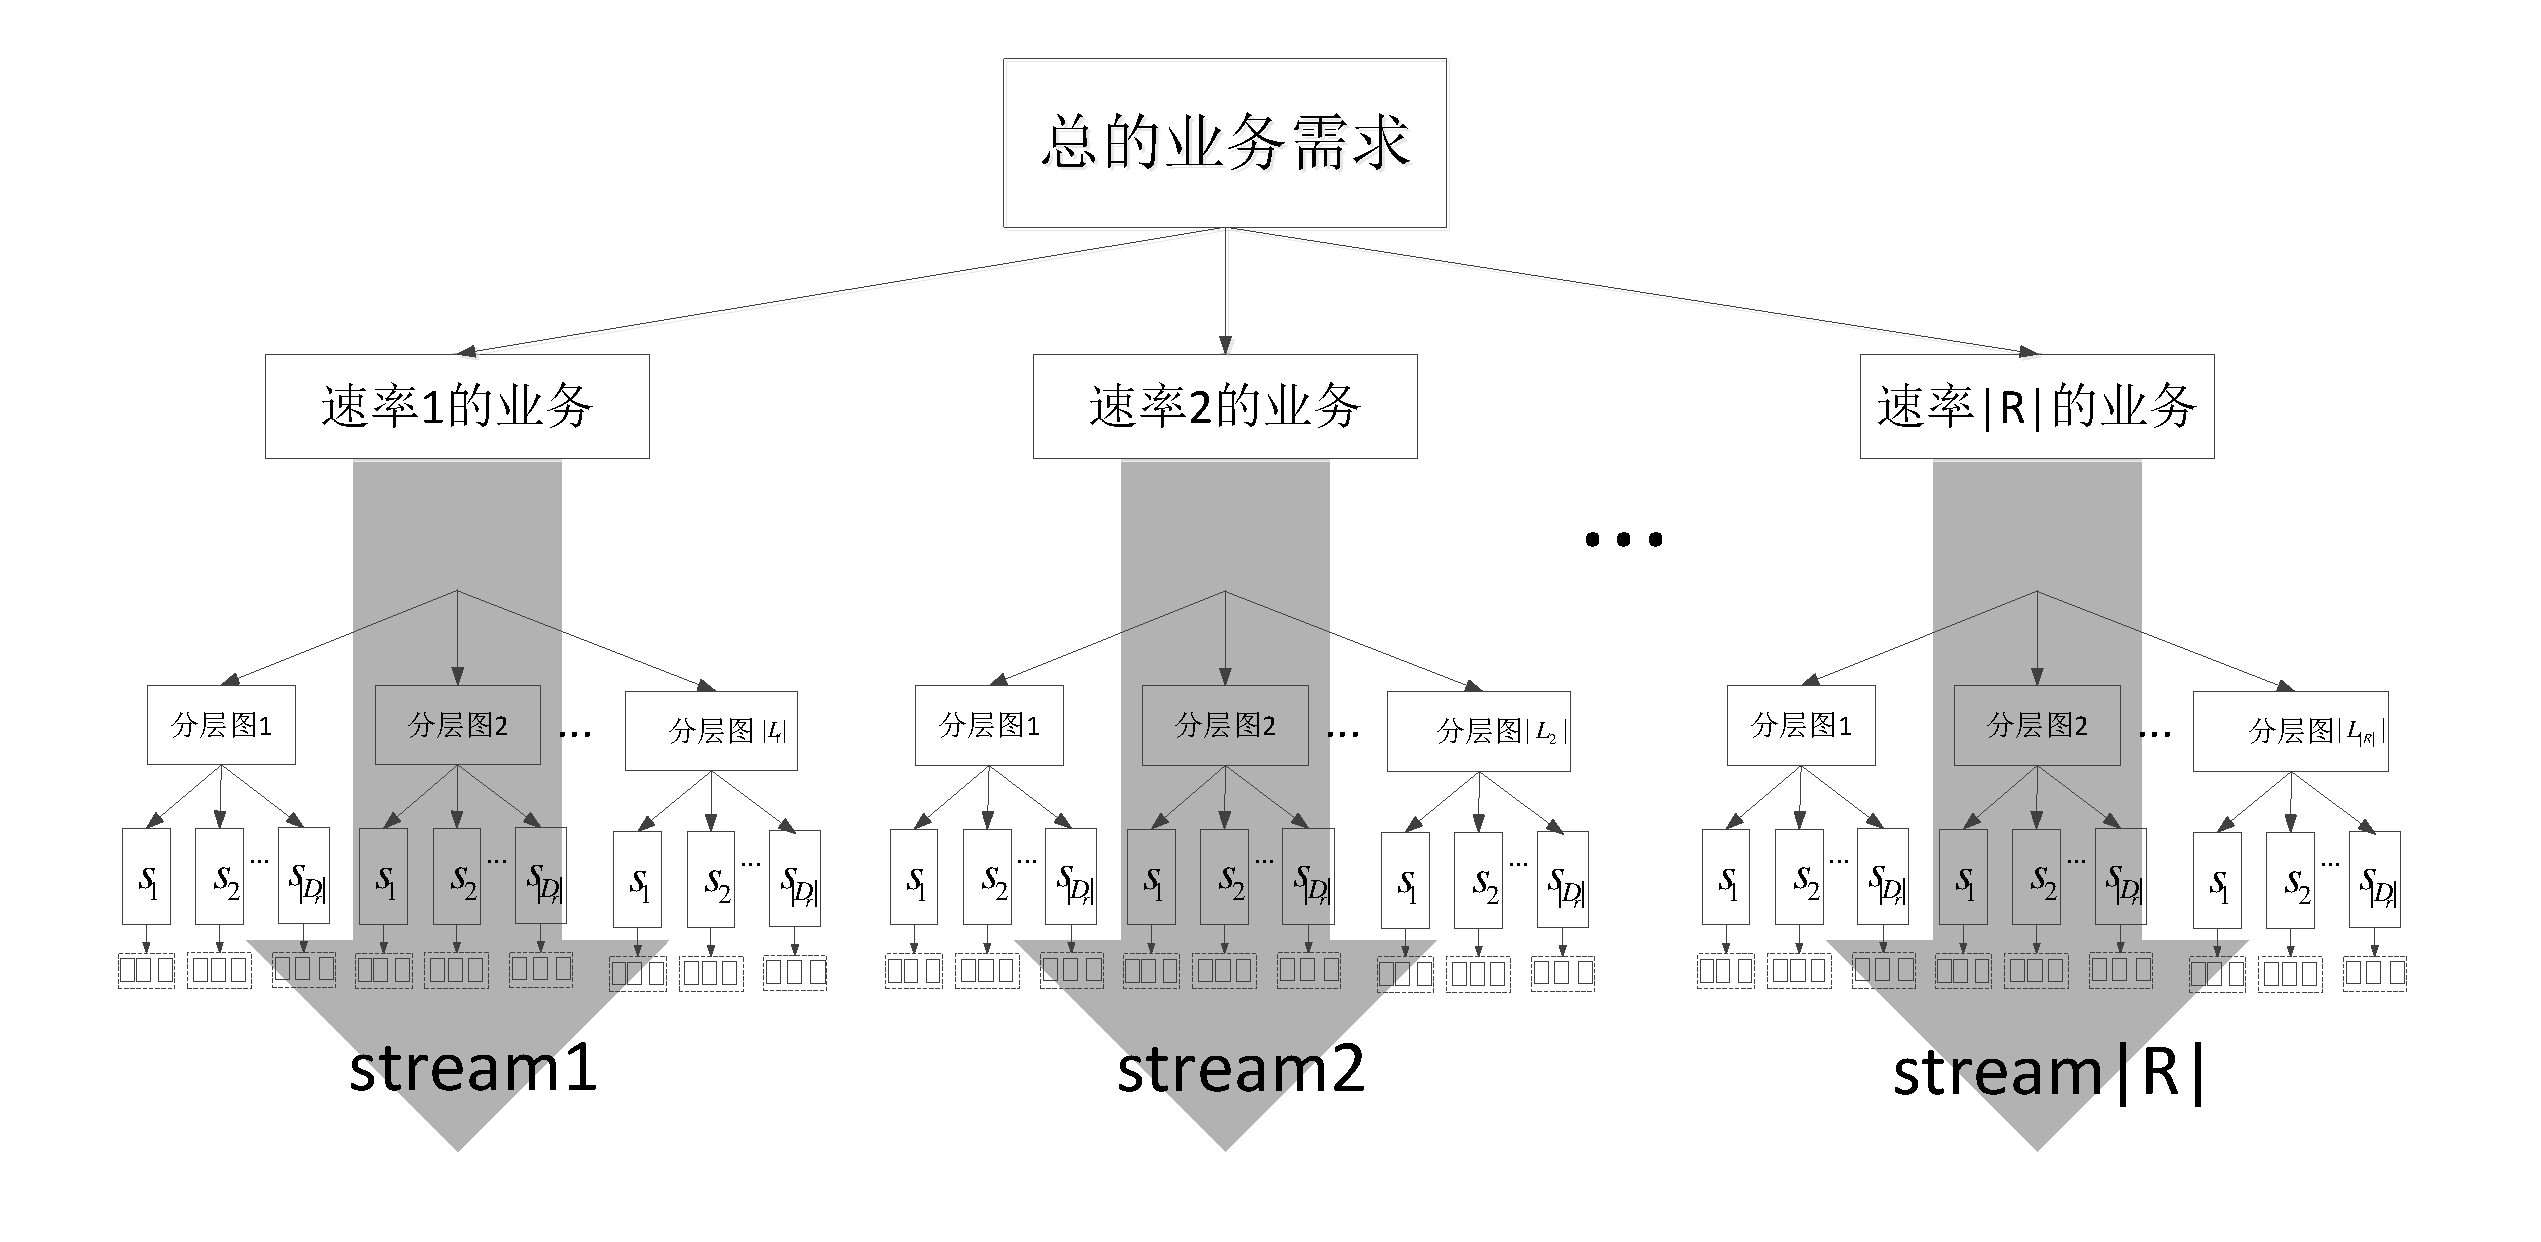
\includegraphics[width=1 \textwidth]{figures/hbfs.pdf}}
    \end{center}
  \caption{{\footnotesize{bfs流并行示意图}}}
  \label{bfssteam}
\end{figure*}
 我们为每一个速率建立一个stream来负责这个速率的业务计算,假设业务一个有$|R|$个不同速率,那么需要建立$|R|$个stream,多个kernel同时执行,充分利用GPU的SMIT资源,当SIMT资源足够时,每个kernel将并行执行,当SIMIT不足时,不同的kernel之间可以进行快速的切换,以达到隐藏延迟的效果。另外,每个速率的内部业务计算的并行如()所讨论的那样。
\subsection{kernel设计}
  和**中讨论不一样,在bfs的并行中不会存在前驱节点更新的同步问题,但是,我们依然需要两个kernel函数,这是因为扩展kernel需要执行多次,如果扩展和更新同时执行,那么更新也会执行多次,这会增多内存访问,所以我们把两个操作分成两个kernel,一个$kernel_bfs_extend$进行边的扩展操作,一个$kernel_bfs_update$进行前驱节点的更新操作,其中$kernel_bfs_extend$需要多次调用,但是$kernel_bfs_update$只需要在最后执行一次。
\begin{algorithm}[t]
\begin{algorithmic}[1]
\caption{\small{kernel\_bfs\_extend($E$, $Dist$,$rid$,$round$)}}
\label{KernelBFS}
\State {$bid \leftarrow$ block ID}
\State {$tid \leftarrow$ thread ID}
\State {用$(bid,tid,rid)$ 映射到边的标号$eid$}
\State {用$(bid,tid,rid)$ 映射到分层图标号$lid$}
\State {$e \leftarrow E[gid][eid]$}
\If {$e.avaliable==-1$}
\State{return}
\EndIf
\State {用$(bid,tid,rid)$ 映射到的源点标号$sid$}
\If{$Dist[lid][sid][e.head]>round&&Dist[lid][sid][e.tail]+1==round$}
\State {$Dist[gid][sid][e.head] \leftarrow round$}
\EndIf
\Return
\end{algorithmic}
\end{algorithm} 
 在$kernel_bfs_extend$中,输入$E$是所有的分层图的边所组成的集合,$Dist$是预先分配的距离标记数组,他是一个三维数组,第一维表示当前距离数组对应的分层图标号,第二维度表示源节点,第三维度表示目的节点,比如$Dist[3][10][5]$=4表示在第3个分层图上,点10到3的距离为4,初始时,除了源节点距离被初始化为0之外,其他的距离都被初始化为无穷大。$rid$表示当前kernel负责的计算的业务速率标号,他是区分不同流的标记,$rid$不同表示执行kernel的流不同。$round$表示当前扩展的层数,由于BFS是一层一层进行扩展操作,我们需要记录当前层数来决定哪些边需要扩展。算法开始时先进行一系列映射操作,将线程映射到边标号$eid$,当前所在分层图标号$lid$,以及源节点标号$sid$。由于动态情况下,边的可用状态可能发生变化,找到边之后,需要判断这条边是否可用,如果不可用则返回。接着判断当前边是否可以进行扩展操作,如果尾节点已经更新过了($Dist[lid][sid][e.head]<=round$),则不能再更新了,反之,还需要判断头节点是否上一次扩展层的节点($Dist[lid][sid][e.tail]+1==round$),如果是的话,那么就更新尾节点的距离为当前扩展层$round$。
\begin{algorithm}[t]
\begin{algorithmic}[1]
\caption{\small{kernel\_bfs\_update($E$, $Pre$,$rid$)}}
\label{KernelBFS}
\State {$bid \leftarrow$ block ID}
\State {$tid \leftarrow$ thread ID}
\State {用$(bid,tid,rid)$ 映射到边的标号$eid$}
\State {用$(bid,tid,rid)$ 映射到分层图标号$lid$}
\State {$e \leftarrow E[gid][eid]$}
\If {$e.avaliable==-1$}
\State{return}
\EndIf
\State {用$(bid,tid,rid)$ 映射到的源点标号$sid$}
\If{$Dist[lid][sid][e.head]==Dist[lid][sid][e.tail]+1$}
\State {$Pre[gid][sid][e.head] \leftarrow e.tail$}
\EndIf
\Return
\end{algorithmic}
\end{algorithm} 
 $kernel_bfs_update$
\section{带权图情况下的GPU算法设计}
\subsection{带跳数限制的最短路算法}
\subsection{点并行的bellman-ford算法}
\subsection{并行层次}
\subsection{kernel设计}
\section{实验仿真分析}